\lab{Sparse Grids}{spgrid}
\label{lab:spgrid}

\objective{Sparse Grids are an important tool when dealing with high-dimensional problems.  Computers operate in discrete space, not in continuous space.  It is important to choose evaluation points wisely so as to maximize accuracy without sacrificing computation time.  In particular, we explore how to use sparse grids to compute integrals of high dimensionality.}

\section*{Discretization}
At first inspection, our world appears to be nice and continuous.  However, this only works on a macroscopic level.  As we zoom in on matter, we find that it is made of discrete atoms with much empty space between.  Computers likewise work in discrete space.  You have already seen many examples of this.  Consider plotting the function $y=x^2$, such as in Figure \ref{fig:x_squared}.  To do this we take an array of discrete points of $x$ and $y$ values, which are then joined in a linear manner.  As you either zoom in on the function or decrease the number of plotting points, you can see the discrete nature of even this simple function.

In order to get better results, we need to use a larger number of points.  This is true not just for graphing purposes, but also for standard computation.  If we double the number of points, we approximately double the computation time necessary.  This effect, while not irrelevant, pales in comparison to the case when working in multiple dimensions.  Imagine a function that we discretize into $20$ points.  A similar function of two variables, where each variable is discretized into $20$ points, would necessitate $400$ unique points.  Expanding to seven variables would necessitate $1,280,000,000$ unique points!

In general, for $n$ discrete points in $d$ dimensions, this gives $n^d$ points.  This can be visualized as a $d$-dimensional grid of size $n \times n \times \cdots \times n$. In practice, we seldom need to know the value for each and every point.  Instead of using the full grid, we can use a sparse grid.  The main idea of a sparse grid is that it can reduce the order of difficulty for a standard $d$-dimensional problem.

\begin{center}
\begin{figure}
\begin{subfigure}{.49\textwidth}
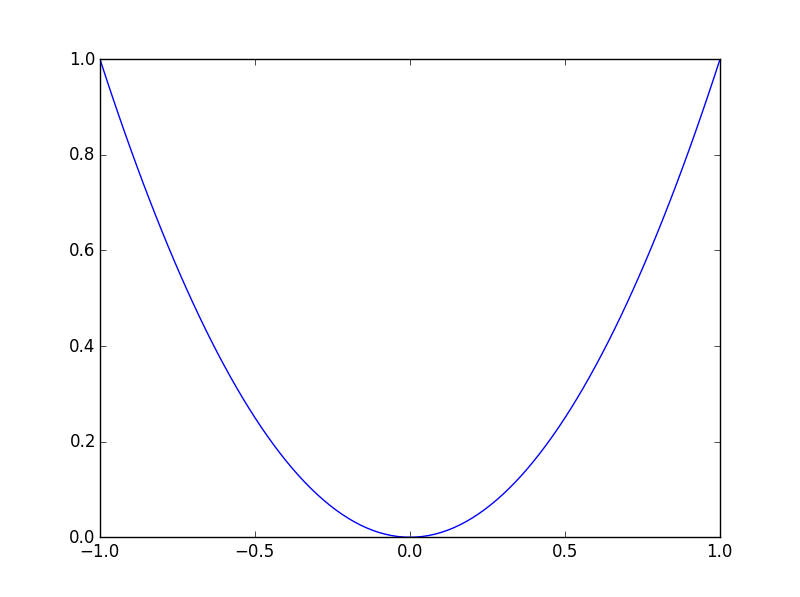
\includegraphics[width=\textwidth]{x2.png}
\end{subfigure}
\begin{subfigure}{.49\textwidth}
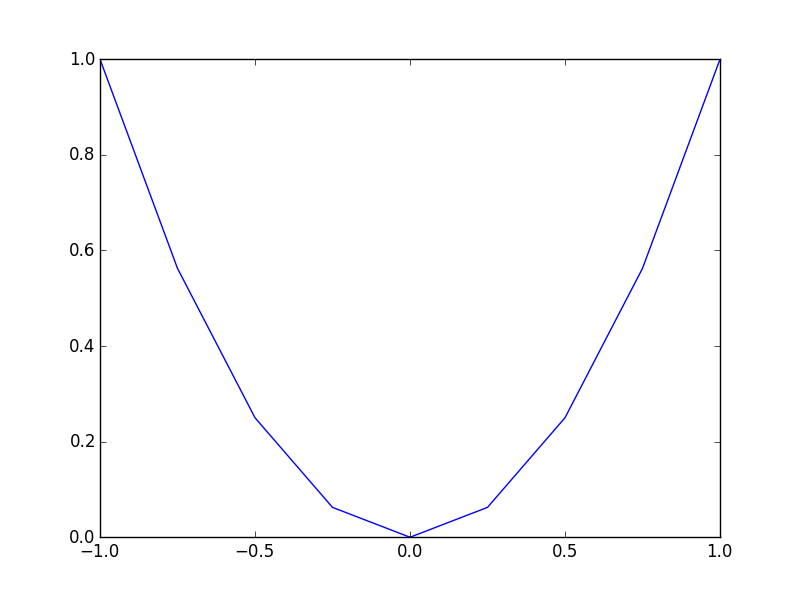
\includegraphics[width=\textwidth]{x2a.png}
\end{subfigure}
\caption{Plots of the function $y=x^2$ using $31$ points and $9$ points, respectively.  In the $9$-point plot, the linear, discrete nature of the function is easily visible.}
\label{fig:x_squared}
\end{figure}
\end{center}

\section*{The Hierarchical Basis}
The basic sparse grid is based on the use of the \emph{Hierarchical Basis}.  This basis is composed of piecewise-linear functions known as the \emph{standard hat functions}, and can be used to approximate any function.  The standard hat function in one dimension is defined as:

\begin{equation}
\phi(x) = \left\{
        \begin{array}{ll}
            1-\abs{x} & \quad -1 \leq x \leq 1 \\
            0 & \quad otherwise
        \end{array}
    \right.
\end{equation}

From this equation, we can build the set of basis functions of order $j$

\begin{equation}
\phi_{j,i}(x) = \phi(2^{j-1}(x+1) - 2i+1)
\end{equation}

\begin{center}
where $i=1,2,3,\cdots,2^{j-1}$.  
\end{center}

The first few basis functions are listed in Table \ref{table:functions}, and are plotted in Figure \ref{fig:basis_functions}.

\begin{center}
\begin{figure}
\begin{subfigure}{.49\textwidth}
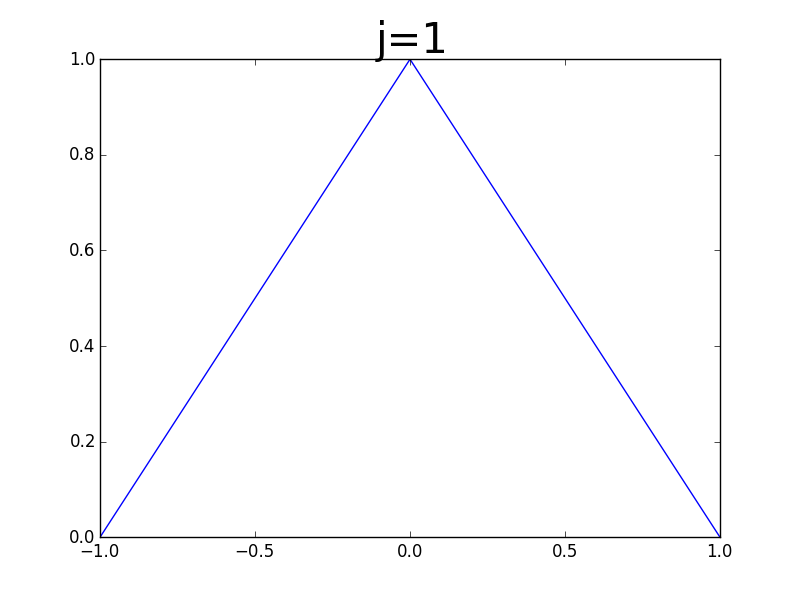
\includegraphics[width=\textwidth]{j1.png}
\end{subfigure}
\begin{subfigure}{.49\textwidth}
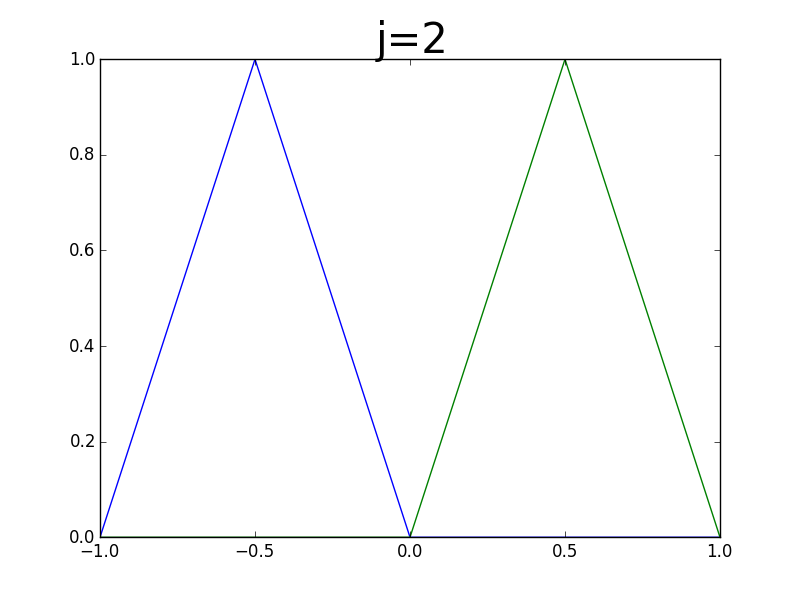
\includegraphics[width=\textwidth]{j2.png}
\end{subfigure}
\begin{subfigure}{.49\textwidth}
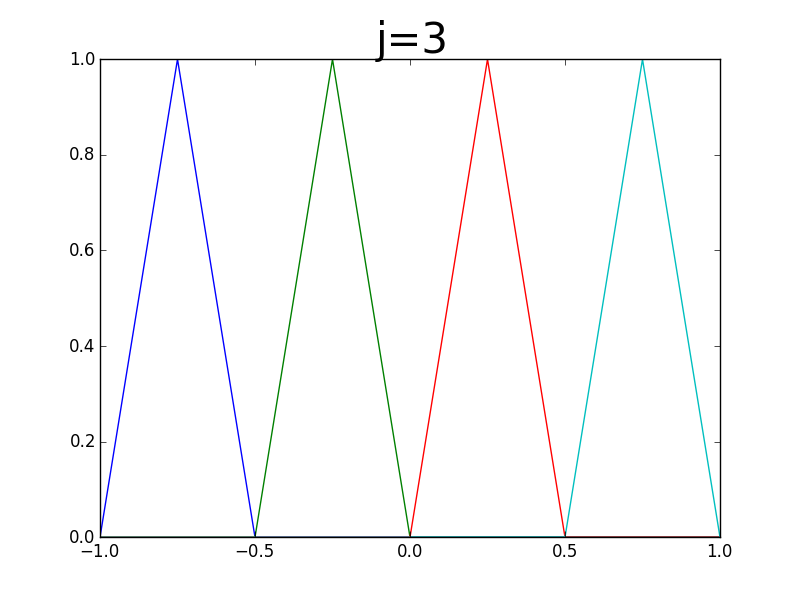
\includegraphics[width=\textwidth]{j3.png}
\end{subfigure}
\begin{subfigure}{.49\textwidth}
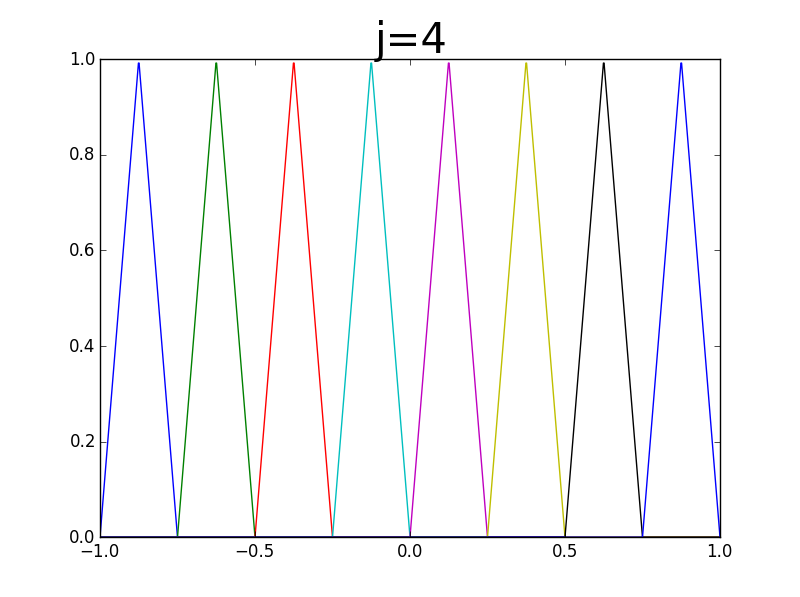
\includegraphics[width=\textwidth]{j4.png}
\end{subfigure}
\caption{Plots of the first few standard hat functions.  Note that the value of $j$ gives the number of ``hats" in the domain $[-1,1]$, and $i$ gives which hat, counting from the left-most hat.}
\label{fig:basis_functions}
\end{figure}
\end{center}

\begin{center}
\begin{table}
\begin{center}
\begin{tabular}{|c|c|c|c|c|}
\hline
$j\backslash i$ & $1$ & $2$ & $3$  & max $i$ \\ \hline
$1$ & $\phi_{11}(x) = \phi(x)$ & & & 1 \\ \hline
$2$ & $\phi_{21}(x) = \phi(2x+1)$ & $\phi_{22}(x) = \phi(2x-1)$ & & 2\\ \hline
$3$ & $\phi_{31}(x) = \phi(4x+3)$ & $\phi_{32}(x) = \phi(4x+1)$ & $\phi_{33}(x) = \phi(4x-1)$ & 4 \\ \hline
$4$ & $\phi_{41}(x) = \phi(8x+7)$ & $\phi_{42}(x) = \phi(8x+5)$ & $\phi_{43}(x) = \phi(8x+3)$ & 8 \\ \hline
$5$ & $\phi_{51}(x) = \phi(16x+15)$ & $\phi_{52}(x) = \phi(16x+13)$ & $\phi_{53}(x) = \phi(16x+11)$ & 16 \\ \hline
\end{tabular}
\caption{The first few standard hat functions that make up the hierarchical basis, for $i\leq3$.}
\label{table:functions}
\end{center}
\end{table}
\end{center}

Using these basis functions, we can approximate any function of our choosing.  Suppose we want to solve
\begin{equation*}
\int_{-1}^{1} \sqrt{1-x^2}\: dx .
\end{equation*}
This is the area of a semi-circle of radius $1$, and can easily be computed mathematically as $\pi / 2 \approx 1.57079632679$.  But a computer does not calculate this in the same manner.  Instead, it uses certain points to evaluate the integral numerically.  We can approximate $f(x) = \sqrt{1-x^2}$ by interpolating the basis hat functions.  If we approximate up to order $l$ then this gives
\begin{equation*}
f(x) \approx \sum_{n=1}^l \sum_{m=1}^{2^{n-1}} c_{nm} \phi_{nm}(x) 
\end{equation*}
where $c_{nm}$ are the apropriate constants which can be found by evaluating the difference between $f(x)$ and the sum of the basis hat functions of lower order at the peak of each hat:
\begin{equation}
c_{nm} = f(p_{nm}) - \sum_{s=1}^{n-1} \sum_{t=1}^{2^{s-1}} c_{st}*\phi_{st}(p_{nm})
\end{equation}
where
\begin{equation}
p_{nm}=2^{2-n}*(m-0.5)-1
\label{eq:points}
\end{equation}
and $p_{nm}$ is the peak of the $m^{th}$ hat of level $n$.  These points will be important because we will use these to create the basic sparse grid.

\begin{center}
\begin{figure}
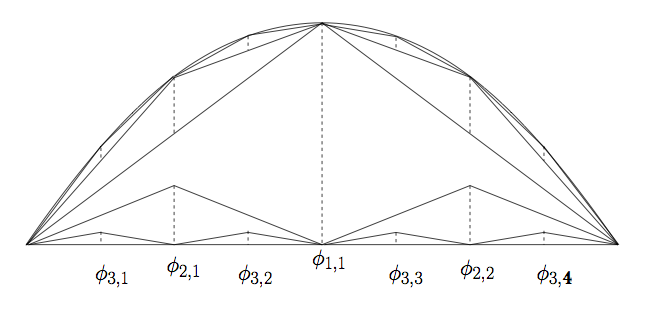
\includegraphics[width=.7\textwidth]{HB.png}
\caption{Interpolating a function using the standard hat basis functions.}
\label{fig:HB}
\end{figure}
\end{center}

One benefit of decomposing $f(x)$ into the basic hat functions is that they are extremely simple to integrate.  Each is a triangle, for which $A=bh/2$.  The height is $1$, and the base is $2^{2-n}$, and so
\begin{equation*}
\int_{-1}^1 \phi_{nm} dx= 2^{1-n}
\end{equation*}

One problem with using the basic hat functions to approximate a function arises when the function does not go to zero at the endpoints.  Higher order approximations yield better results, but ultimately we need to decide how accurate we need our answer to be.  When an additional level changes the answer by less that our error tolerance, we have found a good level of approximation.

 \begin{problem}
Use the function declaration below to approximate a given function on $[-1,1]$ with the basic hat functions up to order $l$:
\begin{lstlisting}
def hat_approximation(f,l):
    """This function will return a list of the correct coefficients to approximate the function f up to level l.
    Parameters
    ----------
        f (function) : The function of a single variable to approximate
        l (int) : The order to use for interpolating the hat function

    Returns
    -------
        coeffs (list) : Entry n is an ndarray of len(2^(n-1)) and contains the coefficients for phi_{nm}.  The length of this should be l.
    """
    pass
\end{lstlisting}
\label{prob:one}
\end{problem}


\begin{center}
\begin{figure}
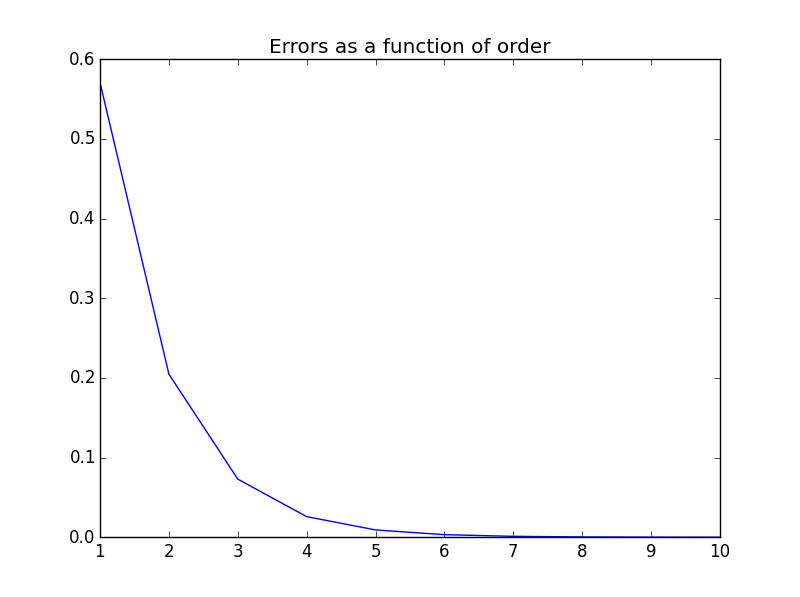
\includegraphics[width=.7\textwidth]{errors.png}
\caption{}
\label{fig:errors}
\end{figure}
\end{center}

\begin{problem}
Write a function that, given the coefficients returned by the function in Problem \ref{prob:one}, returns the value of the integral.

Using the function $f(x)=\sqrt{1-x^2}$, calculate the error of $\int_{-1}^1 f(x)$ in regards to the actual value $\pi/2$.  Do this for the order $l = 1,2,\cdots,10$, and plot the error as a function of $l$.  Your results should match Figure \ref{fig:errors}.  Additionally, time how long it takes to execute the code for each $l$, and plot your results in another graph.
\end{problem}

Keep in mind that thus far we have only used a function of one variable.  For each variable (dimension) the time to compute will increase exponentially.   With multiple dimensions, it becomes infeasible to compute to any degree of accuracy, because the time to compute will increase much too quickly to be reasonable for higher dimensions.  Hence the need for sparse grids.

\section*{Sparse Grids}
Rather than dividing each dimension into $n$ sections, which for $d$ dimensions would give $n^d$ points, sparse grids use only a few of these points.  There are many types of sparse grids, and each is useful for certain purposes.  Which type of sparse grid is used will often depend on the nature of the problem you are trying to solve.  For this lab, we will use the basic sparse grid for purposes of integration.

The basic sparse grid has two main properties, the dimension and the level.  Using these two variables and Equation \ref{eq:points}, we can construct a sparse grid.  Visualizing this in one dimesion is simple: we use as our evaluation points each $p_{nm}$.  A level $1$ grid has one point at the center, which is the peak of the level $1$ hat.  A level $2$ grid has the level $1$ point with two level $2$ points, which are the peaks of the two level $2$ hats.  The third level adds its $4$ points, etc.  So for one dimension of level $l$ we have $\sum_{i=1}^l 2^{i-1}$ points.

Understanding a $2$-dimensional grid  is a bit more complicated.  Our level $1$ point goes at the center of the grid.  To expand to level $2$, we add in the peaks of the level $2$ hats \emph{in both dimensions}, for an additional $4$ points.  Level $3$ is where it gets a little bit tricky mathematically.  We can't just keep expanding only along the axes of the grid, because we need points on the interior as well.  Conceptually, what we do is take our current points and divide the space between points and the end of the grid into two, and there we create a new point.  This is synonymous to adding a hat between the peaks of currently existing points.

We can make a lot more sense of that last paragraph by actually plotting the points.  The file \li{pysg.py} contains a sparse grid class with many useful functions.  Using \li{plotGrid}, you can plot the grid points.  You will first need to create a sparse grid object, and then generate the points using the built in function.  Unfortunately, \li{plotGrid} can only plot up to three dimensions.  Note that in this file, our domain is $[0,1]^d$ rather than $[-1,1]^d$.  
%Be sure to take note of this when computing the integrals in the following problem.  

\begin{problem}
Wrtie a function called \li{points} that takes no inputs and returns an array of size (31, 3), where each row contains the location of a grid point for the $3$-dimensional basic sparse grid of level $3$.
\end{problem}

Multi-dimensional integration for functions with independent endpoints (those that are numbers that do not depend on other variables) is simplified greatly by using sparse grids.  Functions must be manipulated appropriately before sparse grid classes like those in \li{pysg.py} can be used to do the integration, but once this has been done, their evaluation becomes rather simple.  Once the coefficients for the hat functions have been computed, the integrals can be evaluated without having to perform any integration.  Sparse grids are powerful tools for fast computation of high-dimension integrals.  
%In general, note that
%\begin{equation*}
%\int_{a_1}^{b_1} \int_{a_2}^{b_2} \cdots \int_{a_d}^{b_d} \phi_{sii\cdots i}dx_d dx_{d-1} \cdots dx_1= \frac{\prod_{i=1}^d (b_i-a_i)}{2^{(s-1)d}*(d+1)}
%\end{equation*}

%\begin{problem}
%Using the sparse grid class in \li{pysg.py}, compute the value of the following integrals:
%\begin{enumerate}
%\item $\int_{0}^1 \int_{0}^1 (x^2+\frac{1}{3}xy) \ dx dy \ $ to order 8.
%\item $\int_{.36}^{1.8} \int_{0}^{\pi} y*cos(x) \ dx dy \ $ to order 6.
%\item $\int_{-2}^3 \int_{5}^6 \int_{4.2}^{6.3} (\frac{1}{43}x+\frac{1}{123}x^2 y^3 + %\frac{1}{200}yz^2) \ dx dy dz \ $ to order 5.
%\item $\int_{[0,1]^{18}} \prod_{i=1}^{18} x_i \ dx_i \ $ to order 3.
%\end{enumerate}
%\end{problem}